% Options for packages loaded elsewhere
\PassOptionsToPackage{unicode}{hyperref}
\PassOptionsToPackage{hyphens}{url}
\PassOptionsToPackage{dvipsnames,svgnames,x11names}{xcolor}
%
\documentclass[
  oneclumn]{article}

\usepackage{amsmath,amssymb}
\usepackage{iftex}
\ifPDFTeX
  \usepackage[T1]{fontenc}
  \usepackage[utf8]{inputenc}
  \usepackage{textcomp} % provide euro and other symbols
\else % if luatex or xetex
  \usepackage{unicode-math}
  \defaultfontfeatures{Scale=MatchLowercase}
  \defaultfontfeatures[\rmfamily]{Ligatures=TeX,Scale=1}
\fi
\usepackage{lmodern}
\ifPDFTeX\else  
    % xetex/luatex font selection
\fi
% Use upquote if available, for straight quotes in verbatim environments
\IfFileExists{upquote.sty}{\usepackage{upquote}}{}
\IfFileExists{microtype.sty}{% use microtype if available
  \usepackage[]{microtype}
  \UseMicrotypeSet[protrusion]{basicmath} % disable protrusion for tt fonts
}{}
\makeatletter
\@ifundefined{KOMAClassName}{% if non-KOMA class
  \IfFileExists{parskip.sty}{%
    \usepackage{parskip}
  }{% else
    \setlength{\parindent}{0pt}
    \setlength{\parskip}{6pt plus 2pt minus 1pt}}
}{% if KOMA class
  \KOMAoptions{parskip=half}}
\makeatother
\usepackage{xcolor}
\usepackage[left=35mm,right=35mm,top=15mm,bottom=20mm,noheadfoot]{geometry}
\setlength{\emergencystretch}{3em} % prevent overfull lines
\setcounter{secnumdepth}{-\maxdimen} % remove section numbering
% Make \paragraph and \subparagraph free-standing
\ifx\paragraph\undefined\else
  \let\oldparagraph\paragraph
  \renewcommand{\paragraph}[1]{\oldparagraph{#1}\mbox{}}
\fi
\ifx\subparagraph\undefined\else
  \let\oldsubparagraph\subparagraph
  \renewcommand{\subparagraph}[1]{\oldsubparagraph{#1}\mbox{}}
\fi


\providecommand{\tightlist}{%
  \setlength{\itemsep}{0pt}\setlength{\parskip}{0pt}}\usepackage{longtable,booktabs,array}
\usepackage{calc} % for calculating minipage widths
% Correct order of tables after \paragraph or \subparagraph
\usepackage{etoolbox}
\makeatletter
\patchcmd\longtable{\par}{\if@noskipsec\mbox{}\fi\par}{}{}
\makeatother
% Allow footnotes in longtable head/foot
\IfFileExists{footnotehyper.sty}{\usepackage{footnotehyper}}{\usepackage{footnote}}
\makesavenoteenv{longtable}
\usepackage{graphicx}
\makeatletter
\def\maxwidth{\ifdim\Gin@nat@width>\linewidth\linewidth\else\Gin@nat@width\fi}
\def\maxheight{\ifdim\Gin@nat@height>\textheight\textheight\else\Gin@nat@height\fi}
\makeatother
% Scale images if necessary, so that they will not overflow the page
% margins by default, and it is still possible to overwrite the defaults
% using explicit options in \includegraphics[width, height, ...]{}
\setkeys{Gin}{width=\maxwidth,height=\maxheight,keepaspectratio}
% Set default figure placement to htbp
\makeatletter
\def\fps@figure{htbp}
\makeatother
% definitions for citeproc citations
\NewDocumentCommand\citeproctext{}{}
\NewDocumentCommand\citeproc{mm}{%
  \begingroup\def\citeproctext{#2}\cite{#1}\endgroup}
\makeatletter
 % allow citations to break across lines
 \let\@cite@ofmt\@firstofone
 % avoid brackets around text for \cite:
 \def\@biblabel#1{}
 \def\@cite#1#2{{#1\if@tempswa , #2\fi}}
\makeatother
\newlength{\cslhangindent}
\setlength{\cslhangindent}{1.5em}
\newlength{\csllabelwidth}
\setlength{\csllabelwidth}{3em}
\newenvironment{CSLReferences}[2] % #1 hanging-indent, #2 entry-spacing
 {\begin{list}{}{%
  \setlength{\itemindent}{0pt}
  \setlength{\leftmargin}{0pt}
  \setlength{\parsep}{0pt}
  % turn on hanging indent if param 1 is 1
  \ifodd #1
   \setlength{\leftmargin}{\cslhangindent}
   \setlength{\itemindent}{-1\cslhangindent}
  \fi
  % set entry spacing
  \setlength{\itemsep}{#2\baselineskip}}}
 {\end{list}}
\usepackage{calc}
\newcommand{\CSLBlock}[1]{\hfill\break\parbox[t]{\linewidth}{\strut\ignorespaces#1\strut}}
\newcommand{\CSLLeftMargin}[1]{\parbox[t]{\csllabelwidth}{\strut#1\strut}}
\newcommand{\CSLRightInline}[1]{\parbox[t]{\linewidth - \csllabelwidth}{\strut#1\strut}}
\newcommand{\CSLIndent}[1]{\hspace{\cslhangindent}#1}

\usepackage{inputenc}
\makeatletter
\@ifpackageloaded{caption}{}{\usepackage{caption}}
\AtBeginDocument{%
\ifdefined\contentsname
  \renewcommand*\contentsname{Table of contents}
\else
  \newcommand\contentsname{Table of contents}
\fi
\ifdefined\listfigurename
  \renewcommand*\listfigurename{List of Figures}
\else
  \newcommand\listfigurename{List of Figures}
\fi
\ifdefined\listtablename
  \renewcommand*\listtablename{List of Tables}
\else
  \newcommand\listtablename{List of Tables}
\fi
\ifdefined\figurename
  \renewcommand*\figurename{Figure}
\else
  \newcommand\figurename{Figure}
\fi
\ifdefined\tablename
  \renewcommand*\tablename{Table}
\else
  \newcommand\tablename{Table}
\fi
}
\@ifpackageloaded{float}{}{\usepackage{float}}
\floatstyle{ruled}
\@ifundefined{c@chapter}{\newfloat{codelisting}{h}{lop}}{\newfloat{codelisting}{h}{lop}[chapter]}
\floatname{codelisting}{Listing}
\newcommand*\listoflistings{\listof{codelisting}{List of Listings}}
\makeatother
\makeatletter
\makeatother
\makeatletter
\@ifpackageloaded{caption}{}{\usepackage{caption}}
\@ifpackageloaded{subcaption}{}{\usepackage{subcaption}}
\makeatother
\ifLuaTeX
  \usepackage{selnolig}  % disable illegal ligatures
\fi
\usepackage{bookmark}

\IfFileExists{xurl.sty}{\usepackage{xurl}}{} % add URL line breaks if available
\urlstyle{same} % disable monospaced font for URLs
\hypersetup{
  colorlinks=true,
  linkcolor={blue},
  filecolor={Maroon},
  citecolor={Blue},
  urlcolor={Blue},
  pdfcreator={LaTeX via pandoc}}

\author{}
\date{}

\begin{document}

\section{Universidade Federal de
Pernambuco}\label{universidade-federal-de-pernambuco}

\vspace{-.4cm}

\section{Centro de Ciências Exatas e da
Natureza}\label{centro-de-ciuxeancias-exatas-e-da-natureza}

\vspace{-.4cm}

\section{Departamento de
Estatística}\label{departamento-de-estatuxedstica}

\vspace{.5cm}

\subsection{TÓPICOS ESPECIAIS EM ESTATÍSTICA
COMPUTACIONAL}\label{tuxf3picos-especiais-em-estatuxedstica-computacional}

\vspace{.5cm}

\subsubsection{Titulo: Predição de Níveis de Renda usando Redes Neurais:
Análise Comparativa de Técnicas de
Regularização}\label{titulo-prediuxe7uxe3o-de-nuxedveis-de-renda-usando-redes-neurais-anuxe1lise-comparativa-de-tuxe9cnicas-de-regularizauxe7uxe3o}

\vspace{.5cm}

\subsection{María José García
Montes}\label{maruxeda-josuxe9-garcuxeda-montes}

\textbf{Data:} 06 de diciembre de 2025

\vspace{.5cm}

\section{Abstract}\label{abstract}

Este estudo investiga a eficácia de redes neurais totalmente conectadas
na predição de níveis de renda com base em características demográficas
e laborais. Utilizando o Adult Census Dataset (\(32.561\) observações),
foram implementadas e comparadas duas arquiteturas: uma rede neural
simples e outra incorporando técnicas de dropout para regularização. Os
resultados demonstram que a arquitetura com dropout alcançou desempenho
superior em termos de generalização, reduzindo significativamente o
overfitting em \(11.14%
\) e obtendo \(85.71%
\) de acurácia nos dados de teste, em comparação com \(81.97%
\) do modelo simples.

Palavras-chave: Redes Neurais, Dropout, Modelo Simple

\section{Introdução}\label{introduuxe7uxe3o}

A predição de níveis de renda baseada em características individuais
constitui um problema relevante tanto no âmbito acadêmico quanto
aplicado. Modelos precisos podem auxiliar em políticas públicas,
segmentação de mercado e estudos socioeconômicos. Tradicionalmente,
técnicas estatísticas como regressão logística têm sido empregadas para
esta finalidade, porém redes neurais artificiais emergem como
alternativas promissoras devido à sua capacidade de capturar relações
não-lineares complexas.

O desafio central no emprego de redes neurais reside na tendência ao
overfitting, especialmente em conjuntos de dados com dimensionalidade
elevada e relações complexas entre variáveis. A técnica de dropout,
introduzida por Srivastava et al.~(2014), surge como uma solução
elegante e eficaz para este problema, promovendo a aprendizagem de
representações mais robustas através da desativação aleatória de
neurônios durante o treinamento.

Este trabalho tem como objetivo principal comparar o desempenho de redes
neurais totalmente conectadas com e sem dropout na predição de níveis de
renda utilizando o Adult Census Dataset. Especificamente, busca-se: (i)
implementar ambas as arquiteturas; (ii) avaliar métricas de desempenho
comparativas

\section{Fundamentação Teórica}\label{fundamentauxe7uxe3o-teuxf3rica}

\subsection{Redes Neurais Artificiais}\label{redes-neurais-artificiais}

As redes neurais artificiais consistem em unidades de processamento
interconectadas (neurônios) organizadas em camadas sequenciais. Para um
problema de classificação binária, como a predição de renda, a função de
ativação na camada de saída utiliza tipicamente a função sigmoide:

\[\sigma(z) = \frac{1}{1 + e^{-z}}\]

onde \(z\) epresenta a combinação linear das entradas da camada anterior
Segundo (Hastie, Tibshirani, and Friedman 2009)

\subsection{Redes Neuronais Totalmente
Conectadas}\label{redes-neuronais-totalmente-conectadas}

Uma rede neural totalmente conectada (Multilayer Perceptron -- MLP) é
composta por camadas densas, nas quais cada neurônio se conecta a todos
os neurônios da camada seguinte. Matematicamente, uma camada oculta pode
ser representada como:

\[
\mathbf{H} = \varphi(\mathbf{X}\mathbf{W}^{(1)} + \mathbf{b}^{(1)})
\]

e a saida como:

\[
\mathbf{O} = \varphi(\mathbf{H}\mathbf{W}^{(2)} + \mathbf{b}^{(2)})
\]

onde \(\varphi(\cdot)\) é uma função de ativação não linear,
\(\mathbf{H}\) representa o vetor de entradas,\(\mathbf{W}^{(2)}\) os
pesos da primeira camada e \(\mathbf{b}^{(2)}\) o vetor de vieses. A
composição de múltiplas camadas permite aproximar funções complexas e
modelar interações não lineares entre variáveis, segundo (Ferreira
2025c)

\subsection{Overfitting}\label{overfitting}

O overfitting ocorre quando um modelo aprende ruídos e padrões
específicos do conjunto de treinamento, degradando seu desempenho em
dados não vistos. Em redes profundas, o elevado número de parâmetros
aumenta esse risco, especialmente quando as variáveis são numerosas ou
apresentam colinearidade e ruído, segundo (Ferreira 2025a)

\subsection{Dropout como Técnica de
Regularização}\label{dropout-como-tuxe9cnica-de-regularizauxe7uxe3o}

O Dropout é uma técnica que ``desativa'' aleatoriamente neurônios
durante o treinamento com uma probabilidade \(𝑝\). Esse processo força a
rede a aprender representações mais robustas e distribuídas, reduzindo a
coadaptação entre neurônios. Conceitualmente, o Dropout pode ser
interpretado como um ensemble implícito de múltiplas sub-redes, o que
melhora a capacidade de generalização. Durante a fase de inferência,
todas as neurônios são ativados, segundo (Srivastava et al. 2014)

\subsection{Matriz de Confusão e Métricas de
Avaliação}\label{matriz-de-confusuxe3o-e-muxe9tricas-de-avaliauxe7uxe3o}

Para problemas de classificação binária como a predição de níveis de
renda, a \textbf{matriz de confusão} é uma ferramenta importante para
avaliar o desempenho do modelo Ferreira (2025b).

\section{Aplicação}\label{aplicauxe7uxe3o}

Utilizou-se o Adult Census Dataset, disponível no repositório da UCI
Machine Learning, composto por \(32.561\) observações e \(15\)
variáveis, de las cuales \(6\) son variables numericas, \(8\) variables
categoricas e a variável resposta é income, categorizada em dois níveis:
\(<=50K\) e \(>50K\)

\subsection{Análise Exploratória}\label{anuxe1lise-exploratuxf3ria}

Como se observa na Figure~\ref{fig-distribucion-ingresos}, existe um
desequilíbrio significativo na distribuição dos níveis de renda, em que
\(24.720\) observações pertencem ao nível de renda inferior \((<=50K)\),
enquanto apenas \(7.841\) se encontram no nível superior \((>50K)\).

\begin{figure}

\centering{

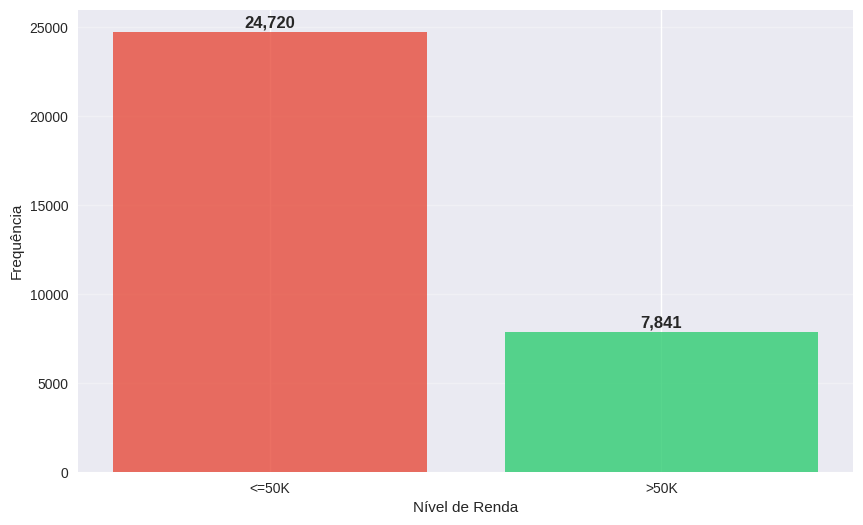
\includegraphics[width=0.7\textwidth,height=\textheight]{descargaa.png}

}

\caption{\label{fig-distribucion-ingresos}Distribuiçao dos Níveis de
Renda.}

\end{figure}%

\begin{minipage}{\textwidth}
\centering
\vspace{-10pt}
\footnotesize \textit{Fonte: Elaboração própria}
\end{minipage}

Além disso, a composição demográfica revela uma distribuição desigual
por gênero, com predominância masculina de \(66.9%
\) (\(21.790\) homens) em comparação com \(33.1%
\) de representação feminina (\(10.771\) mulheres).

Também se verificou que os indivíduos com maiores rendas apresentaram
características distintivas: idade média de \(44.2\) anos e nível
educacional médio de \(11.6\) anos de educação formal. Essas
estatísticas refletem tendências consistentes com a literatura
socioeconômica, na qual a experiência laboral acumulada e a educação
formal estão positivamente associadas a níveis mais elevados de renda.

Para lidar com o desbalanceamento de classes encontrado, foram criadas
duas redes neurais com a mesma estrutura de \(4\) camadas
(\(256-128-64-32\) neurônios), mas em uma delas foram adicionadas
camadas de dropout progressivo (\(50%-40%-30%-20%
\)). Ambas foram treinadas com o otimizador Adam durante 100 épocas,
utilizando o conjunto de treinamento (\(80%
\) dos dados) para o aprendizado e reservando os \(20%
\) restantes para validação, o que permitiu comparar especificamente se
o dropout auxilia o modelo a generalizar melhor em dados.

\subsection{Avaliação do Desempenho
Preditivo}\label{avaliauxe7uxe3o-do-desempenho-preditivo}

A análise comparativa revelou diferenças significativas no desempenho
entre ambas as arquiteturas. Como se apresenta na
Table~\ref{tbl-distribucion}, o modelo com dropout demonstrou
superioridade consistente em todas as métricas avaliadas.

A melhoria mais notável foi observada na precisão \((+9.17%)
\), indicando que o modelo regularizado é significativamente mais
confiável ao prever a classe minoritária \((>50K)\). O F1-Score, que
equilibra precisão e recall, apresentou uma melhoria de \(6.0%
\), refletindo um equilíbrio geral mais adequado na classificação.

\begin{longtable}[]{@{}llll@{}}
\caption{Comparación de métricas entre
arquitecturas}\label{tbl-distribucion}\tabularnewline
\toprule\noalign{}
Métrica & Red Simple & Red com Dropout & Melhora \\
\midrule\noalign{}
\endfirsthead
\toprule\noalign{}
Métrica & Red Simple & Red com Dropout & Melhora \\
\midrule\noalign{}
\endhead
\bottomrule\noalign{}
\endlastfoot
\textbf{Accuracy} & 81.97\% & \textbf{85.71\%} & \textbf{+3.74\%} \\
\textbf{Precisão} & 63.47\% & \textbf{72.64\%} & \textbf{+9.17\%} \\
\textbf{Recall} & 59.18\% & \textbf{65.18\%} & \textbf{+6.0\%} \\
\textbf{F1-Score} & 61.25\% & \textbf{68.71\%} & \textbf{+7.46\%} \\
\textbf{AUC-ROC} & 0.8691 & \textbf{0.9063} & \textbf{+0.0372} \\
\textbf{Loss} & 1.1812 & \textbf{0.3440} & \textbf{-0.8372} \\
\end{longtable}

\begin{center}
\footnotesize \textit{Fonte: Elaboração própria}
\end{center}

Na Table~\ref{tbl-overfitting}, observam-se padrões distintivos na
capacidade de generalização de ambas as arquiteturas. A rede neural
simples apresenta um comportamento de sobreajuste: embora tenha
alcançado \(95.35%
\) de precisão nos dados de treinamento, seu desempenho reduziu-se para
\(81.97%
\) na validação, refletindo uma diferença de \(13.38%
\) entre os dois conjuntos. Essa discrepância sugere que o modelo
capturou ruídos e padrões específicos do conjunto de treinamento,
comprometendo sua aplicabilidade a dados novos.

Em contraste, a rede com dropout demonstrou um perfil de aprendizado
substancialmente mais robusto. Como se observa na Tabela
Table~\ref{tbl-overfitting}, embora tenha apresentado uma precisão de
treinamento mais moderada \((87.94%)
\), manteve um desempenho consistentemente elevado na validação
\((85.71%)
\), reduzindo a diferença de sobreajuste para apenas \(2.24%
\). Essa melhoria de \(11.14\) pontos percentuais em generalização,
combinada com um ganho de \(3.74\) pontos em precisão preditiva real,
valida a efetividade do dropout como mecanismo de regularização.

A estratégia evidencia que, em problemas de classificação com dados
complexos, priorizar a capacidade de generalização, mesmo à custa de um
desempenho ligeiramente inferior no treinamento, resulta em modelos mais
confiáveis e com maior aplicabilidade em cenários reais.

\begin{longtable}[]{@{}llll@{}}
\caption{Análisis de overfitting entre
arquitecturas}\label{tbl-overfitting}\tabularnewline
\toprule\noalign{}
Métrica & Red Simple & Red com Dropout & Melhora \\
\midrule\noalign{}
\endfirsthead
\toprule\noalign{}
Métrica & Red Simple & Red com Dropout & Melhora \\
\midrule\noalign{}
\endhead
\bottomrule\noalign{}
\endlastfoot
\textbf{Accuracy Entrenamiento} & 95.35\% & 87.94\% & -7.41\% \\
\textbf{Accuracy Validación} & 81.97\% & \textbf{85.71\%} &
\textbf{+3.74\%} \\
\textbf{Overfitting} & 13.38\% & \textbf{2.24\%} & \textbf{-11.14\%} \\
\end{longtable}

\begin{center}
\footnotesize \textit{Fonte: Elaboração própria}
\end{center}

Na \hyperref[fig-accuracy-asc]{Figura 2a}, o modelo simples evidencia
sobreajuste, refletido em uma diferença considerável entre as curvas de
accuracy de treinamento e validação. Enquanto o treinamento alcança
aproximadamente \(95%
\), a validação se estabiliza em torno de \(81.9%
\), o que indica baixa capacidade de generalização. Em contraste, o
modelo que incorpora a técnica de Dropout demonstra curvas mais estáveis
e próximas entre si, alcançando um accuracy de validação final de
\(85.7%
\). Esses resultados confirmam a efetividade da regularização por
Dropout na melhoria do desempenho preditivo da rede neural.

Este resultado se confirma na \hyperref[fig-loss-bkl]{Figura 2b}, onde o
modelo simples apresenta aumento da perda em validação, enquanto a perda
em treinamento continua diminuindo, evidenciando a ocorrência de
sobreajuste. Em contraste, o modelo com aplicação da técnica de Dropout
mantém ambas as curvas descendentes e próximas entre si, indicando um
processo de treinamento mais estável e com maior capacidade de
generalização.

\begin{longtable}[]{@{}
  >{\raggedright\arraybackslash}p{(\columnwidth - 2\tabcolsep) * \real{0.5000}}
  >{\raggedright\arraybackslash}p{(\columnwidth - 2\tabcolsep) * \real{0.5000}}@{}}
\toprule\noalign{}
\endhead
\bottomrule\noalign{}
\endlastfoot
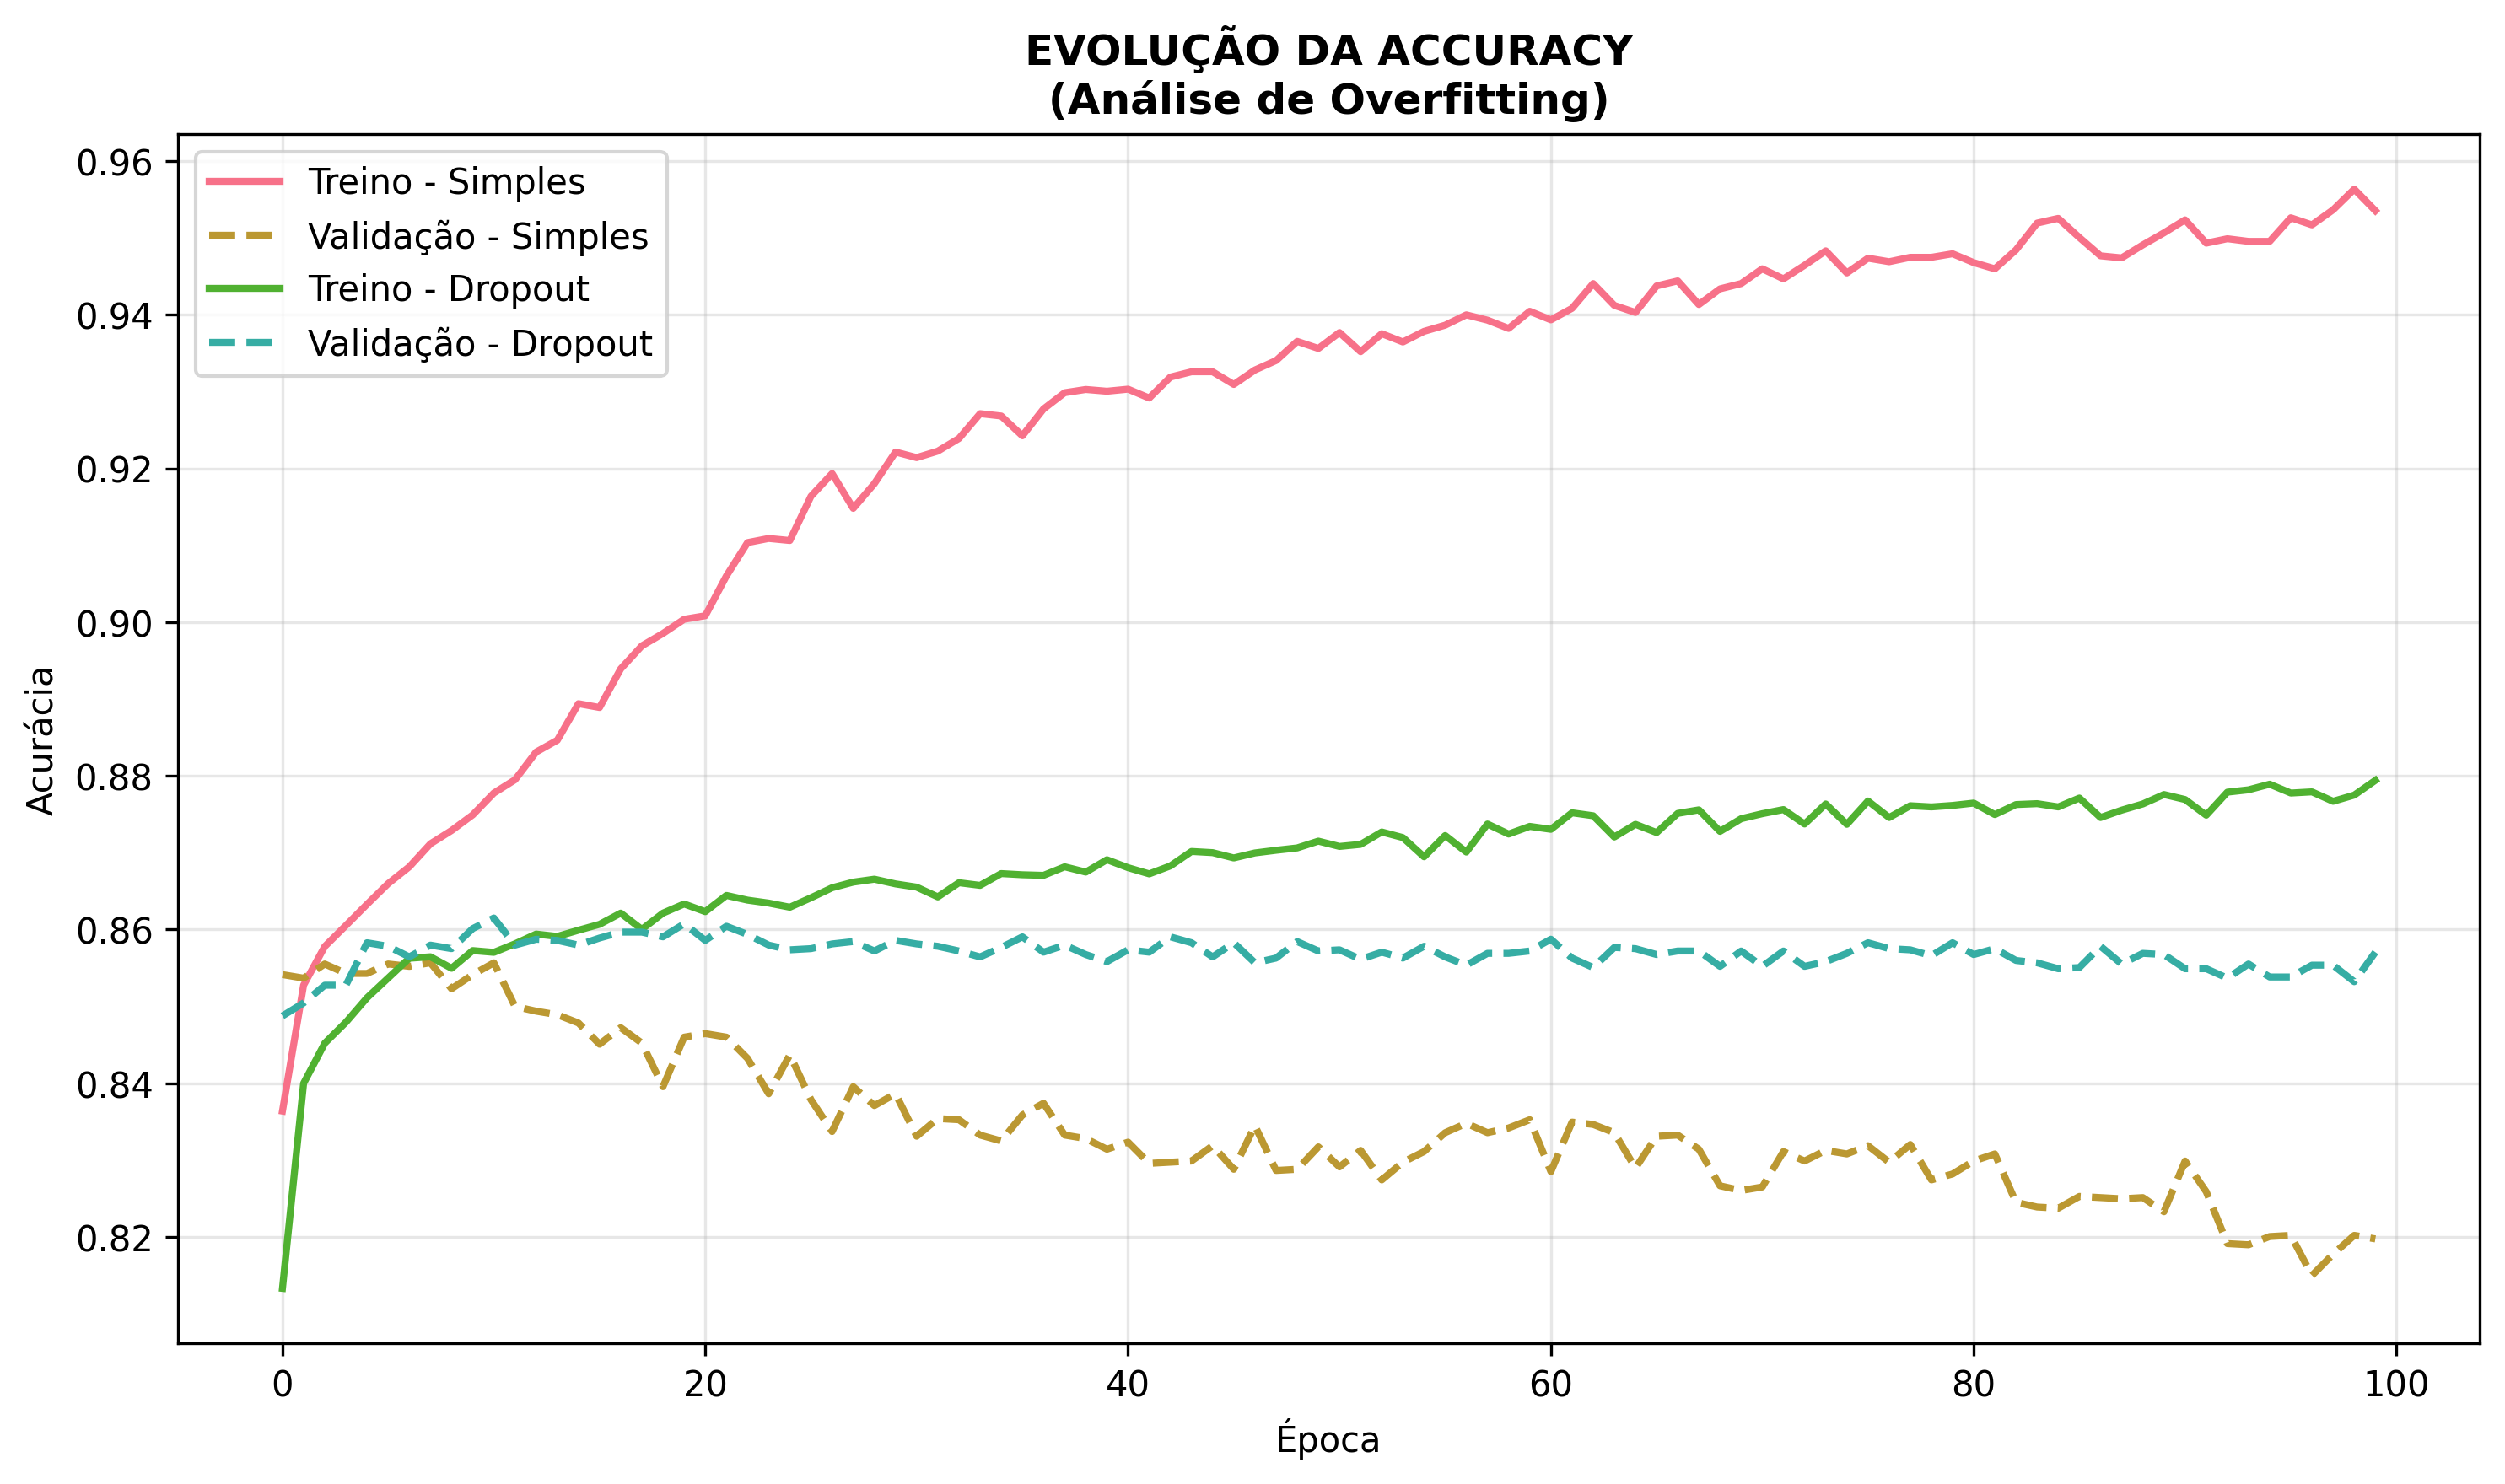
\includegraphics[width=0.49\textwidth,height=\textheight]{evolucao_accuracy.png}
&
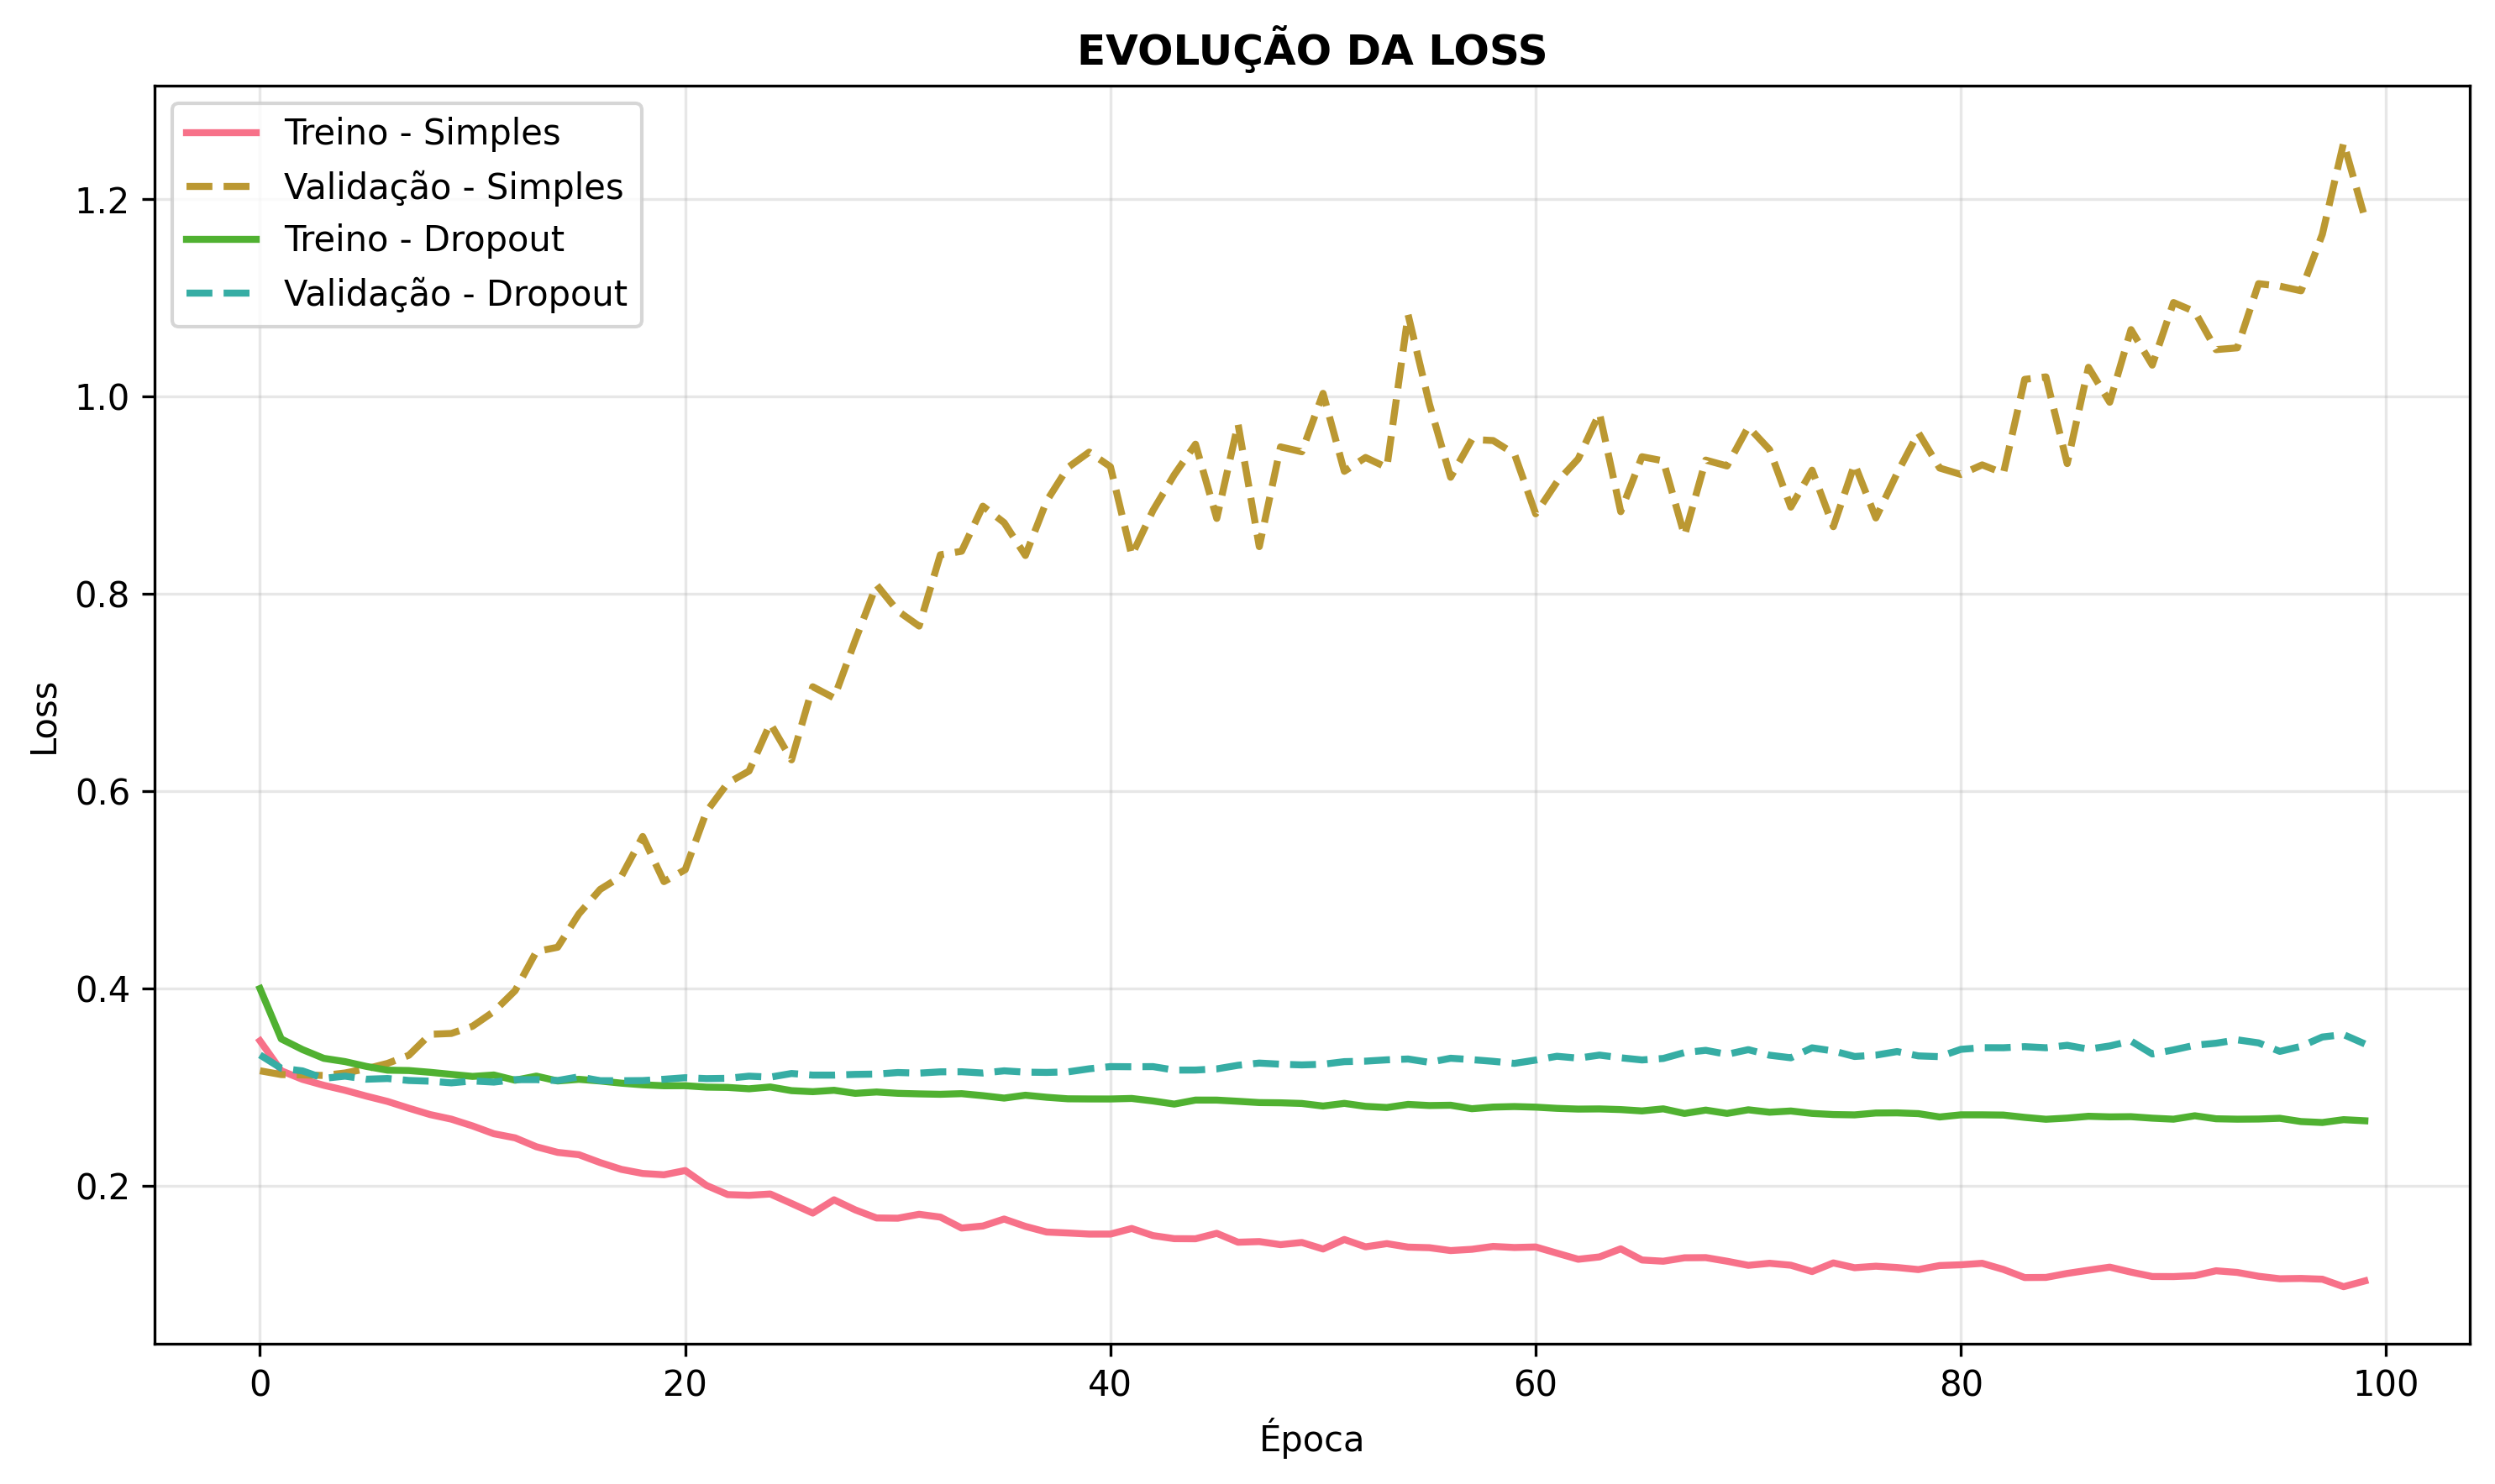
\includegraphics[width=0.49\textwidth,height=\textheight]{evolucao_loss.png} \\
\textbf{Figura 2a:} Evolución de la Accuracy & \textbf{Figura 2b:}
Evolución de la Loss \\
\end{longtable}

\begin{center}
\footnotesize \textit{Fonte: Elaboração própria}
\end{center}

A Figure~\ref{fig-roc-comparativa} apresenta as curvas ROC
correspondentes a ambos os modelos. Observa-se que o modelo com
aplicação da técnica de Dropout exibe uma curva que se mantém
consistentemente acima da curva do modelo simples, indicando uma maior
taxa de verdadeiros positivos para um mesmo nível de falsos positivos.

Além disso, a curva do modelo com Dropout aproxima-se de forma mais
consistente do lado superior esquerdo do gráfico, região que representa
uma classificação ideal. O valor da AUC confirma essa superioridade, com
\(0.906\) em comparação a \(0.869\), evidenciando uma maior capacidade
de discriminação entre as classes.

\begin{figure}

\centering{

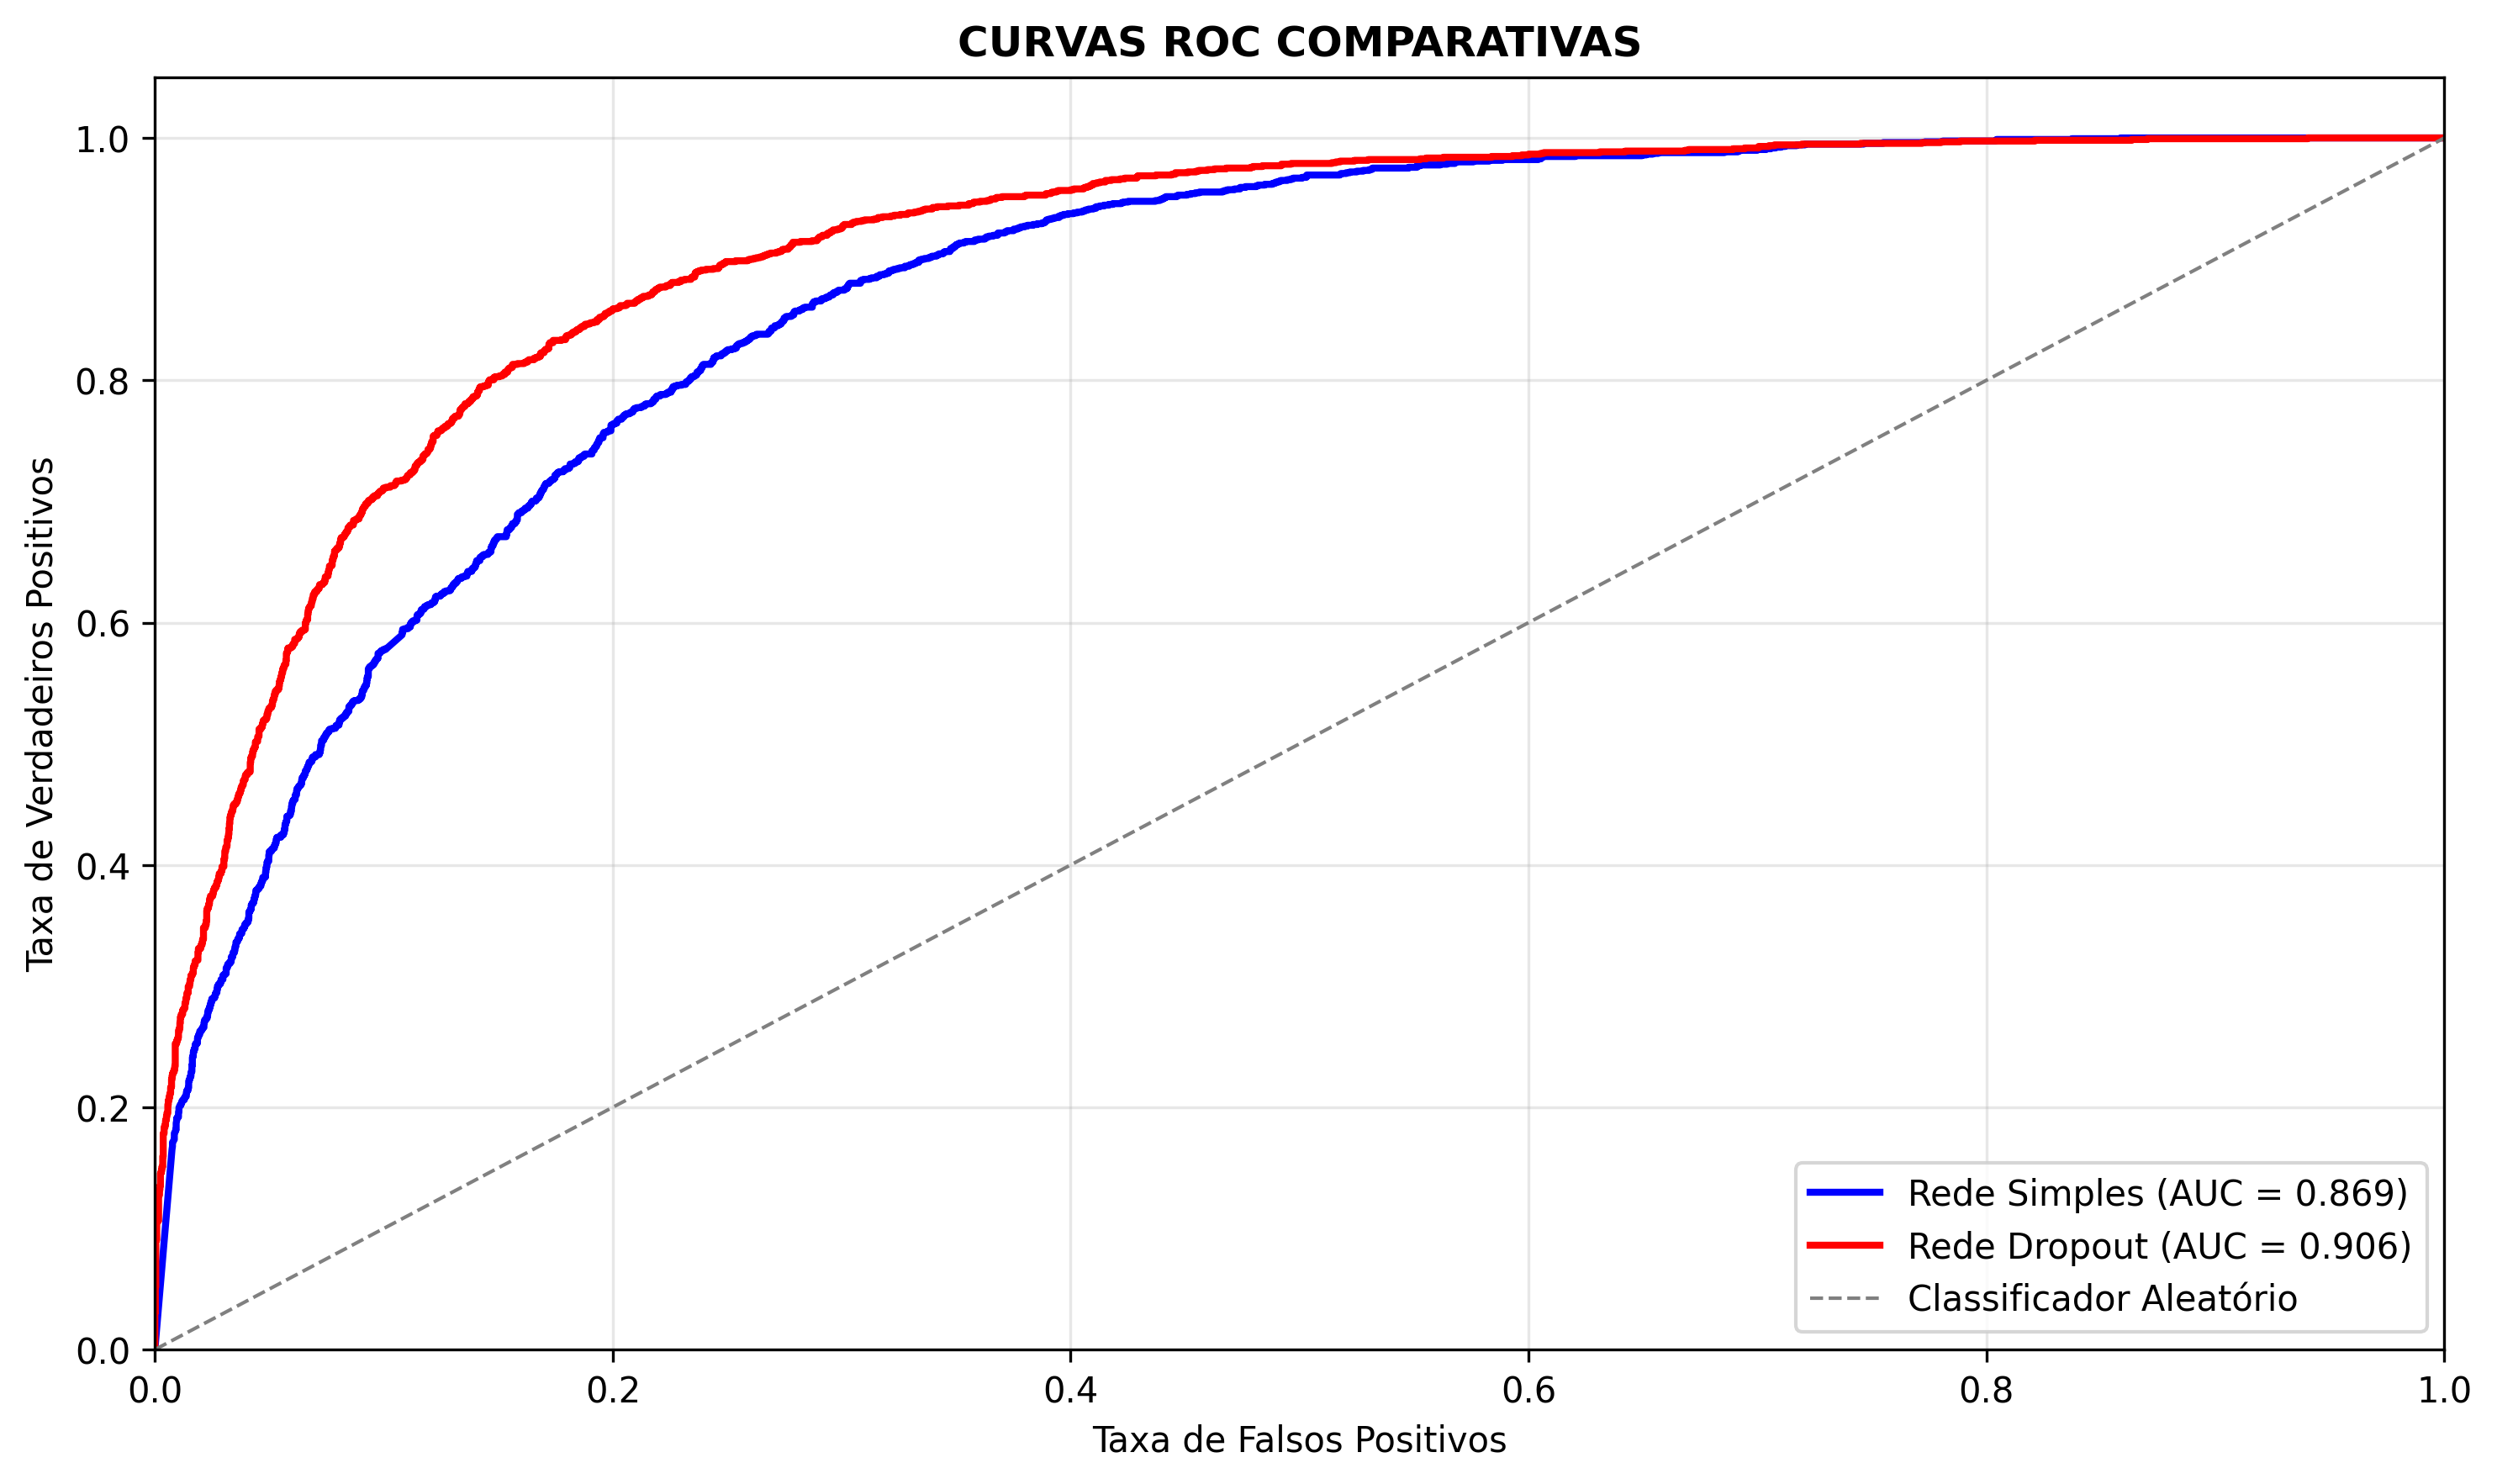
\includegraphics[width=0.7\textwidth,height=\textheight]{curvas_roc.png}

}

\caption{\label{fig-roc-comparativa}Evaluação da Accuracy}

\end{figure}%

\begin{minipage}{\textwidth}
\centering
\vspace{-10pt}
\footnotesize \textit{Fonte: Elaboração própria}
\end{minipage}

Na tabela Table~\ref{tbl-overfittinghtyugf}, observa-se que o modelo
simples identifica corretamente \(4.411\) instâncias da classe
majoritária \((<=50K)\), o que representa uma taxa de acerto de \(89,20%
\). No entanto, para a classe minoritária \((>50K)\), o modelo acerta
apenas \(928\) dos \(1.568\) casos reais, resultando em uma taxa de
acerto de \(59,18%
\).

\begin{longtable}[]{@{}
  >{\raggedright\arraybackslash}p{(\columnwidth - 8\tabcolsep) * \real{0.1667}}
  >{\centering\arraybackslash}p{(\columnwidth - 8\tabcolsep) * \real{0.2083}}
  >{\centering\arraybackslash}p{(\columnwidth - 8\tabcolsep) * \real{0.2083}}
  >{\centering\arraybackslash}p{(\columnwidth - 8\tabcolsep) * \real{0.2083}}
  >{\centering\arraybackslash}p{(\columnwidth - 8\tabcolsep) * \real{0.2083}}@{}}
\caption{Matriz de Confusão - Modelo
Simple}\label{tbl-overfittinghtyugf}\tabularnewline
\toprule\noalign{}
\begin{minipage}[b]{\linewidth}\raggedright
Valor Real ~Valor Predito
\end{minipage} & \begin{minipage}[b]{\linewidth}\centering
\textbf{\textless=50K}
\end{minipage} & \begin{minipage}[b]{\linewidth}\centering
\textbf{\textgreater50K}
\end{minipage} & \begin{minipage}[b]{\linewidth}\centering
\textbf{Total}
\end{minipage} & \begin{minipage}[b]{\linewidth}\centering
\textbf{Tasa de Acierto}
\end{minipage} \\
\midrule\noalign{}
\endfirsthead
\toprule\noalign{}
\begin{minipage}[b]{\linewidth}\raggedright
Valor Real ~Valor Predito
\end{minipage} & \begin{minipage}[b]{\linewidth}\centering
\textbf{\textless=50K}
\end{minipage} & \begin{minipage}[b]{\linewidth}\centering
\textbf{\textgreater50K}
\end{minipage} & \begin{minipage}[b]{\linewidth}\centering
\textbf{Total}
\end{minipage} & \begin{minipage}[b]{\linewidth}\centering
\textbf{Tasa de Acierto}
\end{minipage} \\
\midrule\noalign{}
\endhead
\bottomrule\noalign{}
\endlastfoot
\textbf{\textless=50K} & 4.411 & 534 & 4,945 & \textbf{89.20\%} \\
\textbf{\textgreater50K} & 640 & 928 & 1,568 & \textbf{59.18\%} \\
\textbf{Total} & 5,051 & 1,462 & 6,513 & \\
\textbf{Precisión por Clase} & \textbf{87.33\%} & \textbf{63.48\%} & &
\textbf{Accuracy Global: 81.97\%} \\
\end{longtable}

\begin{center}
\footnotesize \textit{Fonte: Elaboração própria}
\end{center}

Na tabela Table~\ref{tbl-overfittinghtyugfIKL}, o modelo com Dropout
melhora em ambas as classes: \(+3,01%
\) na classe majoritária e \(+5,99%
\) na minoritária.

\begin{longtable}[]{@{}
  >{\raggedright\arraybackslash}p{(\columnwidth - 8\tabcolsep) * \real{0.1667}}
  >{\centering\arraybackslash}p{(\columnwidth - 8\tabcolsep) * \real{0.2083}}
  >{\centering\arraybackslash}p{(\columnwidth - 8\tabcolsep) * \real{0.2083}}
  >{\centering\arraybackslash}p{(\columnwidth - 8\tabcolsep) * \real{0.2083}}
  >{\centering\arraybackslash}p{(\columnwidth - 8\tabcolsep) * \real{0.2083}}@{}}
\caption{Matriz de Confusão - Modelo com
Dropout}\label{tbl-overfittinghtyugfIKL}\tabularnewline
\toprule\noalign{}
\begin{minipage}[b]{\linewidth}\raggedright
Valor Real ~Valor Predito
\end{minipage} & \begin{minipage}[b]{\linewidth}\centering
\textbf{\textless=50K}
\end{minipage} & \begin{minipage}[b]{\linewidth}\centering
\textbf{\textgreater50K}
\end{minipage} & \begin{minipage}[b]{\linewidth}\centering
\textbf{Total}
\end{minipage} & \begin{minipage}[b]{\linewidth}\centering
\textbf{Tasa de Acierto}
\end{minipage} \\
\midrule\noalign{}
\endfirsthead
\toprule\noalign{}
\begin{minipage}[b]{\linewidth}\raggedright
Valor Real ~Valor Predito
\end{minipage} & \begin{minipage}[b]{\linewidth}\centering
\textbf{\textless=50K}
\end{minipage} & \begin{minipage}[b]{\linewidth}\centering
\textbf{\textgreater50K}
\end{minipage} & \begin{minipage}[b]{\linewidth}\centering
\textbf{Total}
\end{minipage} & \begin{minipage}[b]{\linewidth}\centering
\textbf{Tasa de Acierto}
\end{minipage} \\
\midrule\noalign{}
\endhead
\bottomrule\noalign{}
\endlastfoot
\textbf{\textless=50K} & 4,560 & 385 & 4,945 & \textbf{92.21\%} \\
\textbf{\textgreater50K} & 546 & 1,022 & 1,568 & \textbf{65.17\%} \\
\textbf{Total} & 5,106 & 1,407 & 6,513 & \\
\textbf{Precisión por Clase} & \textbf{89.31\%} & \textbf{72.64\%} & &
\textbf{Accuracy Global: 85.71\%} \\
\end{longtable}

\begin{center}
\footnotesize \textit{Fonte: Elaboração própria}
\end{center}

\section{Conclusão}\label{conclusuxe3o}

Os resultados obtidos ao longo deste estudo evidenciam que o modelo
simples apresenta limitações significativas, refletidas na discrepância
entre as curvas de treinamento e validação, no aumento da perda durante
a validação e no desempenho inferior em métricas como accuracy e AUC.
Esses achados confirmam a ocorrência de limitações, comprometendo a
capacidade preditiva do modelo quando aplicado a novos dados.

Em contraste, o modelo com Dropout demonstrou maior estabilidade ao
longo do processo de treinamento, apresentando curvas de desempenho mais
próximas entre si e métricas superiores. O aumento consistente do
accuracy de validação, a redução da perda e a superioridade tanto da
curva ROC quanto do valor de AUC (\(0.906\) em comparação a \(0.869\))
confirmam a efetividade de dropout na melhoria da capacidade de
discriminação entre classes.

Assim, conclui-se que a aplicação de Dropout, é importante para o
desempenho de redes neurais na tarefa de predição de níveis de renda,
garantindo maior robustez e confiabilidade dos resultados.

\section{Referências}\label{referuxeancias}

\phantomsection\label{refs}
\begin{CSLReferences}{1}{0}
\bibitem[\citeproctext]{ref-ferreira2025dropout}
Ferreira, Jodavid. 2025a. {``Dropout.''}

\bibitem[\citeproctext]{ref-ferreira2025metricas}
---------. 2025b. {``Matriz de Confusão e Métricas de Avaliação.''}
\url{https://jodavid.github.io/computationalstatisticstopics/}.

\bibitem[\citeproctext]{ref-ferreira2025mlp}
---------. 2025c. {``Redes Neurais Totalmente Conectadas.''}

\bibitem[\citeproctext]{ref-hastie2009}
Hastie, Trevor, Robert Tibshirani, and Jerome Friedman. 2009. \emph{The
Elements of Statistical Learning}. Springer New York.
\url{https://doi.org/10.1007/978-0-387-84858-7}.

\bibitem[\citeproctext]{ref-srivastava2014dropout}
Srivastava, Nitish, Geoffrey Hinton, Alex Krizhevsky, Ilya Sutskever,
and Ruslan Salakhutdinov. 2014. {``Dropout: A Simple Way to Prevent
Neural Networks from Overfitting.''} \emph{Journal of Machine Learning
Research} 15: 1929--58.

\end{CSLReferences}



\end{document}
